\section{How Monte Carlo errors compound in particle filters}
\label{sec:pf_errors}

Each step of a particle filter adds Monte Carlo error, and the error of the next step is computed from an already approximate input. Whether these errors accumulate, and how fast, is the central question of sequential Monte Carlo. West~\cite{west1993} approximated posterior distributions by mixtures obtained by kernel smoothing of weighted samples, with the sequential updating of Monte Carlo approximations in view. Liu and West~\cite{liuwest2001} describe the difficulty that such updating brings, the degrading accuracy of particle representations updated over time, as particle attrition under resampling and weight degeneracy under reweighting. Doucet, Godsill and Andrieu~\cite{dga2000} gave a systematic treatment of sequential importance sampling and resampling, including the optimal proposal and the degeneracy of the weights.

\subsection{Weight degeneracy without resampling}

Consider sequential importance sampling without resampling for the hidden Markov model with transition density $p(x_s\mid x_{s-1})$ and likelihood $p(y_s\mid x_s)$. A path $x_{0:t}$ is drawn from a causal proposal, $x_0$ from its prior and $x_s\sim q_s(\cdot\mid x_{s-1},y_s)$ afterwards, and carries the weight $w_t = p(x_{0:t}\mid y_{1:t})/q(x_{0:t}\mid y_{1:t}) = \prod_{s\leq t}u_s$ with increments
\[
u_s = \frac{p(y_s\mid x_s)\,p(x_s\mid x_{s-1})}{q_s(x_s\mid x_{s-1},y_s)\,p(y_s\mid y_{1:s-1})}.
\]
Following Kong, Liu and Wong~\cite{klw1994} and Doucet, Godsill and Andrieu~\cite[Proposition~1]{dga2000}, we regard the observations as random variables with their true law, so that the weight is a function of the path and of the data and its variance is the unconditional variance. Let $\mathcal{F}_s$ be generated by $x_{0:s}$ and $y_{1:s}$. Given $\mathcal{F}_{s-1}$ the pair $(x_s,y_s)$ has density $q_s(x_s\mid x_{s-1},y_s)\,p(y_s\mid y_{1:s-1})$, and the integral of $u_s$ against this density over $x_s$ and $y_s$ is $\int p(x_s\mid x_{s-1})\dd x_s = 1$, provided the proposal is positive wherever the numerator of $u_s$ is. Hence $\E[u_s\mid\mathcal{F}_{s-1}] = 1$ and $(w_t)$ is a positive martingale with mean one.

\begin{proposition}[Kong, Liu and Wong]
\label{prop:klw}
Let $(w_t)$ be a positive square integrable martingale with $\E w_t = 1$ and increments $u_t = w_t/w_{t-1}$. Then the variance of the weight is nondecreasing in $t$:
\[
\Var(w_t) = \Var(w_{t-1})+\E\big[w_{t-1}^2\,\Var(u_t\mid\mathcal{F}_{t-1})\big]\geq\Var(w_{t-1}).
\]
If the increments are independent with $\E u_s^2 = 1+\sigma_s^2$ and $\sigma_s^2\geq\sigma^2>0$, then $\E w_t^2\geq(1+\sigma^2)^t$, with equality when $\sigma_s^2 = \sigma^2$ for all $s$, so the effective sample size $N/\E w_t^2$ decays at least geometrically.
\end{proposition}

\begin{proof}
By the martingale property, $\E w_t^2 = \E[w_{t-1}^2\E(u_t^2\mid\mathcal{F}_{t-1})] = \E[w_{t-1}^2(1+\Var(u_t\mid\mathcal{F}_{t-1}))]$, and subtracting $(\E w_t)^2 = 1 = (\E w_{t-1})^2$ gives the identity. If the increments are independent, then $w_{t-1}$ and $u_t$ are independent and $\E w_t^2 = \prod_{s\leq t}\E u_s^2 = \prod_{s\leq t}(1+\sigma_s^2)$.
\end{proof}

The effective sample size cannot increase, and in the model case of the proposition it reaches one after $\log N/\log(1+\sigma^2)$ steps, so that for any fixed $N$ the weights concentrate on a single path, and a larger $N$ postpones the collapse only in proportion to $\log N$. The increments of a hidden Markov model are not independent, but the left panel of Figure~\ref{fig:pf} shows the same geometric decay. It shows the effective sample size $(\sum_iW_i^2)^{-1}$ of the normalized weights $W_i$ for the local level model $x_t = x_{t-1}+\sqrt q\,\varepsilon_t$, $y_t = x_t+\sqrt r\,\nu_t$ with independent standard normal noise, $q = 0.1$, $r = 1$, $x_0\sim N(0,1)$ and $N = 1000$ particles. Without resampling it falls from $1000$ to about $180$ after ten steps, to about $26$ after twenty and to about $4$ after thirty, and it equals one to numerical precision after two hundred. With resampling at every step it stays above $350$.

\subsection{Errors with resampling}

Resampling resets the weights at the price of additional variance and of coalescing genealogies. The hidden state is a Markov chain with transition kernel $M$, and $\eta_1$ is the law of its first state. For a given sequence of observations, $g_t(x) = p(y_t\mid x)$ is the likelihood of the $t$th observation as a function of the state. Write $\eta_t = p(x_t\mid y_{1:t-1})$ for the predictive law, $\pi_t = p(x_t\mid y_{1:t})$ for the filter, $\mu(f) = \int f\dd\mu$, and $\Psi_t(\eta)(\dd x) = g_t(x)\,\eta(\dd x)/\eta(g_t)$ for the map that applies Bayes' rule to a prior $\eta$. Then $\pi_t = \Psi_t(\eta_t)$ and $\eta_{t+1} = \pi_tM = \Phi_t(\eta_t)$, where $\Phi_t(\eta) = \Psi_t(\eta)M$. The bootstrap filter with $N$ particles and multinomial resampling draws $X^1_1,\dots,X^N_1$ independently from $\eta_1$ and forms the empirical measure $\eta^N_t = \frac1N\sum_i\delta_{X^i_t}$ and the weighted measure $\pi^N_t = \Psi_t(\eta^N_t)$. It then draws $N$ ancestors from $\pi^N_t$ and moves each by $M$, so that, given the particles of step $t$, the particles of step $t+1$ are independent with law $\Phi_t(\eta^N_t)$.

\begin{theorem}[Del Moral; Crisan and Doucet; Del Moral and Guionnet]
\label{thm:pf_error}
Suppose that $a^{-1}\leq g_t\leq a$ for all $t$ and some $a\geq1$. Then for every $t$ there is a constant $c_t$ that does not depend on $N$ such that for every bounded $f$,
\[
\E\big|\eta_t^N(f)-\eta_t(f)\big|^2\leq\frac{c_t\,\|f\|_\infty^2}{N},
\]
and the same holds for $\pi_t^N(f)-\pi_t(f)$ with another constant. If in addition $\varepsilon\nu(A)\leq M(x,A)\leq\varepsilon^{-1}\nu(A)$ for all $x$ and all measurable $A$, for some probability $\nu$ and some $\varepsilon\in(0,1]$, then $c_t\leq4a^4\varepsilon^{-8}$ for every $t$: the filter forgets its errors, and the approximation is uniform in time.
\end{theorem}

\begin{proof}
Let $Q_s(x,\dd y) = g_s(x)M(x,\dd y)$, $Q_{s,t} = Q_s\cdots Q_{t-1}$ for $s<t$ and $Q_{t,t}$ the identity, so that $Q_{s,t}f(x)$ is the expectation of $f(X_t)\prod_{s\leq u<t}g_u(X_u)$ for the chain started at $X_s = x$. The exact flow from time $s$ to time $t$ is $\Phi_{s,t} = \Phi_{t-1}\circ\cdots\circ\Phi_s$, with $\Phi_{s,t}(\mu)(f) = \mu(Q_{s,t}f)/\mu(Q_{s,t}1)$ and $\Phi_{s,t}(\eta_s) = \eta_t$. Let $\mathcal{G}_s$ be the history of the particle system up to the particles of step $s$, and put $\bar\eta_1 = \eta_1$ and $\bar\eta_s = \Phi_{s-1}(\eta^N_{s-1})$ for $s\geq2$. Given $\mathcal{G}_{s-1}$ the measure $\eta^N_s$ is the empirical measure of $N$ independent draws from $\bar\eta_s$, and telescoping gives
\[
\eta^N_t(f)-\eta_t(f) = \sum_{s=1}^t\Big(\Phi_{s,t}(\eta^N_s)(f)-\Phi_{s,t}(\bar\eta_s)(f)\Big),
\]
a sum of local errors, the $s$th of which is the sampling error at step $s$ propagated to time $t$ by the exact flow. Write $G = Q_{s,t}1$, let $P_{s,t}f = Q_{s,t}f/G$, a Markov operator, and let $\lambda = \Phi_{s,t}(\bar\eta_s)(f)$. Since $\bar\eta_s(Q_{s,t}f-\lambda G) = 0$, the $s$th local error is
\[
\frac{(\eta^N_s-\bar\eta_s)\big(G\,(P_{s,t}f-\lambda)\big)}{\eta^N_s(G)}.
\]
The constant $\lambda$ is an average of $P_{s,t}f$, so $|P_{s,t}f-\lambda|\leq\omega_{s,t}$, the oscillation $\sup P_{s,t}f-\inf P_{s,t}f$, and $\eta^N_s(G)\geq\inf G$. Dividing by $\sup G\,\omega_{s,t}$ turns $G\,(P_{s,t}f-\lambda)$ into a function $h$ bounded by one, so the local error is at most $(\sup G/\inf G)\,\omega_{s,t}\,|(\eta^N_s-\bar\eta_s)(h)|$. Given $\mathcal{G}_{s-1}$, $(\eta^N_s-\bar\eta_s)(h)$ is the centered mean of $N$ independent variables bounded by one, with second moment at most $1/N$. The local error therefore has $L^2$ norm at most $(\sup G/\inf G)\,\omega_{s,t}\,N^{-1/2}$.

Under the first assumption $a^{-(t-s)}\leq G\leq a^{t-s}$, and $\omega_{s,t}\leq\mathrm{osc}(f)\leq2\|f\|_\infty$ because $P_{s,t}$ is a Markov operator, where $\mathrm{osc}(f) = \sup f-\inf f$. Minkowski's inequality then gives the first claim with $c_t = 4\big(\sum_{k<t}a^{2k}\big)^2$, which grows geometrically in $t$. Under the mixing assumption, $\sup G/\inf G\leq a^2\varepsilon^{-2}$ for $s<t$, because $G = g_sM(Q_{s+1,t}1)$ and $M(Q_{s+1,t}1)(x)$ varies by a factor of at most $\varepsilon^{-2}$ with $x$. Moreover $P_{s,t} = P_{s,s+1}\cdots P_{t-1,t}$ is a product of the Doob transformed kernels $P_{u,u+1}(x,\dd y) = M(x,\dd y)\,Q_{u+1,t}1(y)/M(Q_{u+1,t}1)(x)$, and each satisfies $P_{u,u+1}(x,\cdot)\geq\varepsilon^2\tilde\nu_u$ for all $x$, with $\tilde\nu_u(\dd y)\propto Q_{u+1,t}1(y)\,\nu(\dd y)$. By Dobrushin's contraction argument $\omega_{s,t}\leq(1-\varepsilon^2)^{t-s}\mathrm{osc}(f)$. The $L^2$ norm of the $s$th local error is then at most $a^2\varepsilon^{-2}(1-\varepsilon^2)^{t-s}\mathrm{osc}(f)\,N^{-1/2}$, and the sum over $s$ is at most $a^2\varepsilon^{-4}\mathrm{osc}(f)\,N^{-1/2}$. Finally $\pi^N_t(f)-\pi_t(f) = (\eta^N_t-\eta_t)\big(g_t(f-\pi_t(f))\big)/\eta^N_t(g_t)$ with $\eta^N_t(g_t)\geq a^{-1}$ and $\|g_t(f-\pi_t(f))\|_\infty\leq2a\|f\|_\infty$, so the bounds for $\eta^N_t$ carry over to $\pi^N_t$ with the constants multiplied by $4a^4$.
\end{proof}

The first assertion is the convergence result of Del Moral~\cite{delmoral1998} and of Crisan and Doucet~\cite{crisandoucet2002}, who require only that the likelihoods be bounded. Del Moral and Guionnet~\cite{delmoralguionnet2001} obtained bounds uniform in time, in $L^1$ and with the slower rate $N^{-\alpha/2}$ for some $\alpha<1$, under bounded likelihoods and an exponential stability condition on the filter. C\'erou, Del Moral and Guyader~\cite{cdg2011} state the rate $N^{-1/2}$ uniformly in $t$, as in the second assertion, under a regularity condition of the same kind, and refer to Del Moral's monograph~\cite{delmoral2004} for the convergence analysis of the occupation measures. The Gaussian likelihoods and kernels of the local level model of the figures do not satisfy these bounds, so the theorem describes the mechanism and does not cover that example.

The contraction that does the work in the theorem is a Dobrushin contraction of the Doob transformed kernels of the filter. It depends on the likelihoods as well as on the signal, and it is a different quantity from the spectral gap that governs Markov chain Monte Carlo in Chapter~\ref{ch:ergodic}.

\subsection{The likelihood estimator}

The particle filter also yields an unbiased estimator $\hat p_N(y_{1:t}) = \prod_{s\leq t}\eta^N_s(g_s)$ of the marginal likelihood, the product over time of the average unnormalized weights. Its relative variance compounds. C\'erou, Del Moral and Guyader~\cite{cdg2011} proved a nonasymptotic bound under a regularity condition: the ratio of the largest to the smallest value of each likelihood $g_s$ is at most $\delta$, and for some $m\geq1$ the $m$ step transition kernel satisfies $M^m(x,\cdot)\leq\beta M^m(x',\cdot)$ for all $x$ and $x'$. Under this condition, for $N>(t+1)\beta\delta^m$,
\[
\E\Big[\Big(\frac{\hat p_N(y_{1:t})}{p(y_{1:t})}-1\Big)^2\Big]\leq\frac{4(t+1)\beta\delta^m}{N}
\]
\cite[Corollary~5.2]{cdg2011}. The bound is of order $t/N$. B\'erard, Del Moral and Doucet~\cite{berard2014} showed that this order is correct. Let $t$ and $N$ tend to infinity with $t/N\to\alpha$. Under regularity and stability conditions of the same kind, $\log\hat p_N(y_{1:t})-\log p(y_{1:t})$ converges in law to a normal distribution with mean $-\alpha\sigma^2/2$ and variance $\alpha\sigma^2$, where $\sigma^2$ is a constant of the model. Pitt, Silva, Giordani and Kohn~\cite{pitt2012}, in a study of Markov chain Monte Carlo methods based on the particle filter, conjectured this lognormal limit and gave empirical evidence for it. The variance of the log likelihood estimator is therefore close to $\sigma^2t/N$, and keeping it bounded requires the number of particles to grow linearly with the length of the series. The middle panel of Figure~\ref{fig:pf} shows this for the local level model, where the exact likelihood is available from the Kalman filter: the variance of $\log\hat p_N-\log p$ grows roughly linearly in $t$, and increasing $N$ from $100$ to $1000$ reduces the slope by a factor of about ten.

\begin{figure}[t]
\centering
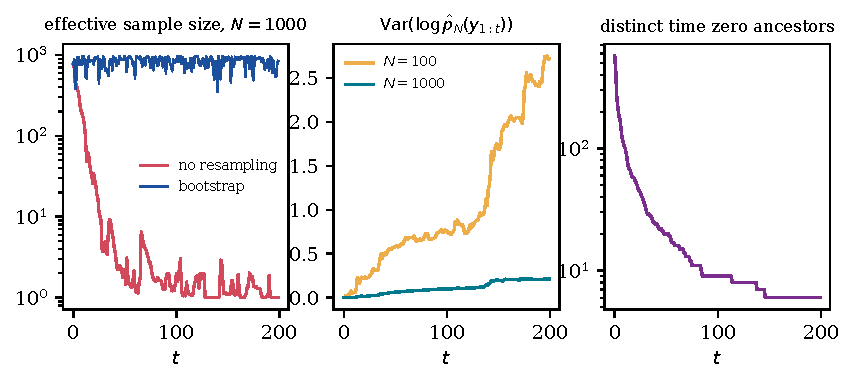
\includegraphics[width=\textwidth]{pf_errors}
\caption{Compounding of Monte Carlo error in particle filters for the local level model with $q = 0.1$ and $r = 1$. Left, effective sample size of the normalized weights for $N = 1000$ particles, with and without resampling. Middle, variance over sixty runs of the log likelihood estimate $\log\hat p_N(y_{1:t})$ for $N = 100$ and $N = 1000$, growing roughly linearly in $t$. Right, on a logarithmic scale, the number of distinct time zero ancestors among the $N = 1000$ resampled particles, the path degeneracy that afflicts smoothing and parameter learning.}
\label{fig:pf}
\end{figure}

\subsection{Path degeneracy and static parameters}

The right panel of Figure~\ref{fig:pf} shows the number of distinct ancestors at time zero of the particles alive at time $t$. It falls from $1000$ to about $570$ after one step, to $105$ after ten, to $20$ after fifty and to $6$ after two hundred. Resampling makes the genealogy coalesce. Two particles chosen at random at step $t$ have the same parent with probability $\sum_iW_i^2$, the inverse of the effective sample size, which is of order $1/N$. Koskela, Jenkins, Johansen and Span\`o~\cite{koskela2020} show, under strong conditions, that the genealogy converges to a Kingman coalescent when time is measured by the accumulated probability of such mergers, so that a single ancestor remains after a number of steps of order $N$. The filtering distribution at time $t$ can still be well approximated, as in Theorem~\ref{thm:pf_error}, but the approximation of the joint smoothing distribution of the whole path by the surviving genealogies is poor at early times. Godsill, Doucet and West~\cite{gdw2004} addressed this with backward simulation smoothing, which reuses the particle approximations of the filtering distributions at all times to draw whole trajectories backward in time, and so does not rely on the forward genealogy.

Static parameters are the worst case. A fixed parameter $\theta$ has no dynamics, so once the particle cloud in $\theta$ degenerates it never recovers, while in a regular model the posterior of $\theta$ keeps contracting at rate $t^{-1/2}$, and Monte Carlo error then dominates statistical error. The remedies developed since are ways of reintroducing dynamics or sufficient statistics: the kernel shrinkage method of Liu and West~\cite{liuwest2001}, which adds an artificial evolution to $\theta$ with the shrinkage rule of West~\cite{west1993} and a variance chosen to preserve the first two moments of the particle cloud; the sufficient statistic particle filters of Storvik~\cite{storvik2002} and of Carvalho, Johannes, Lopes and Polson~\cite{cjlp2010}, which carry conditional sufficient statistics for $\theta$ in each particle; the practical filter of Polson, Stroud and M\"uller~\cite{psm2008}, which approximates the posterior by a mixture of fixed lag smoothing distributions and uses sufficient statistics for the parameters without reweighting particles; and particle Markov chain Monte Carlo~\cite{adh2010}, which embeds the filter inside a Metropolis Hastings chain on $\theta$. Kantas and coauthors~\cite{kantas2015} survey the resulting methods.

\section{The particle filter as an interacting particle system}
\label{sec:pf_interacting}

The particle filter is not only an approximation to one posterior; it is a stochastic process whose time marginals converge, as the number of particles grows, to the predictive laws of the model, and whose reweighted particle clouds converge to the sequence of filtering posteriors. We use the notation of Section~\ref{sec:pf_errors}. Define, for each probability measure $\eta$, the McKean kernel $K_{t,\eta}(x,\cdot) = \Psi_t(\eta)M$, which does not depend on $x$ but depends on $\eta$: a particle at $x$ is replaced by a draw from the updated law and then moved. This is a nonlinear Markov chain in the sense of McKean, the discrete time analogue of the McKean Vlasov processes of Chapter~\ref{ch:kinetic}.

\begin{proposition}[The marginals are the posteriors]
\label{prop:pf_marginals}
Let $\bar X_1\sim\eta_1$ and, recursively, $\bar X_{t+1}\mid\bar X_t\sim K_{t,\mathrm{Law}(\bar X_t)}(\bar X_t,\cdot)$. Then $\mathrm{Law}(\bar X_t) = \eta_t$ for every $t$, and $\Psi_t(\mathrm{Law}(\bar X_t)) = \pi_t$. The time marginals of the nonlinear chain are therefore the predictive laws, and their Bayes updates are the filtering posteriors.
\end{proposition}

\begin{proof}
By induction. If $\mathrm{Law}(\bar X_t) = \eta_t$, then $\mathrm{Law}(\bar X_{t+1}) = \int\eta_t(\dd x)K_{t,\eta_t}(x,\cdot) = \Psi_t(\eta_t)M = \pi_tM = \eta_{t+1}$, and $\Psi_t(\eta_t) = \pi_t$ by Bayes' rule.
\end{proof}

Only the time marginals are asserted. The kernel $K_{t,\eta}(x,\cdot)$ does not depend on $x$, so the values $\bar X_1,\bar X_2,\dots$ are independent, and the law of the path of the chain is the product of the $\eta_t$, not a posterior for the path of the hidden state.

The bootstrap filter is the $N$ particle mean field approximation of this chain: each particle moves by $K_{t,\eta^N_t}$ with the unknown law replaced by the empirical measure $\eta^N_t$. Under the hypotheses of Theorem~\ref{thm:pf_error}, $\eta^N_t$ converges to the deterministic limit $\eta_t$. The particles are exchangeable, so Theorem~\ref{thm:sznitman} shows that the law of each particle at time $t$ converges to $\eta_t$ and that any $k$ particles become independent: the bootstrap filter propagates chaos. A single forward pass with $N$ particles, at cost $O(NT)$, thus delivers approximations to every intermediate posterior $p(x_t\mid y_{1:t})$, $t = 1,\dots,T$, not just the last one (upper panel of Figure~\ref{fig:pl}). Markov chain Monte Carlo, by contrast, targets one posterior at a time and must be rerun when a new observation arrives.

The resampling step selects, for each new particle, an ancestor index $a^i_t\in\{1,\dots,N\}$. These indices are discrete latent variables that switch at every step, and conditionally on the whole ancestry the particles move independently. The particle system is therefore itself a switching model on an extended space, with the ancestor indices as regimes; Andrieu, Doucet and Holenstein used this extended space construction to prove the exactness of particle Markov chain Monte Carlo~\cite{adh2010}. In continuous time the switching structure can be made part of the model itself (Section~\ref{sec:kurtz_xiong}). When the only latent state is a finite regime and the observation densities given the regime are known, the filter is exact and finite dimensional, Hamilton's filter~\cite{hamilton1989}, which is the forward algorithm for hidden Markov models of Section~\ref{sec:wonham}. When the state is linear and Gaussian given the path of the regime, each particle can carry the regime together with the Kalman mean and variance of the continuous state instead of a sampled value. This is the mixture Kalman filter of Chen and Liu~\cite{chenliu2000}, and by the Rao Blackwell inequality $\Var(\E[f\mid s])\leq\Var(f)$ it reduces the variance of the importance weights~\cite{dga2000}. The general principle is that a particle should carry the smallest summary of the past that makes the future conditionally tractable.

\section{Particle learning and conditional sufficient statistics}
\label{sec:particle_learning}

The principle applies to static parameters, where the naive particle filter fails. Suppose the model has parameter $\theta$ and that there are conditional sufficient statistics $s_t$, updated deterministically by
\[
s_{t+1} = S(s_t,x_t,x_{t+1},y_{t+1}),
\]
such that $p(\theta\mid x_{0:t},y_{1:t}) = p(\theta\mid s_t)$. This is the case in conditionally conjugate models, where the posterior of $\theta$ given the states and the data lies in a conjugate family with a sufficient statistic of fixed dimension. An example is the linear Gaussian state space model with unknown variances, treated below. Particle learning, introduced by Carvalho, Johannes, Lopes and Polson~\cite{cjlp2010}, tracks the essential state $z_t = (x_t,s_t,\theta)$ and updates it in a resample and propagate order:
\begin{enumerate}
\item Resample $\{z^i_t\}$ with weights proportional to the predictive likelihood $p(y_{t+1}\mid z^i_t) = \int p(y_{t+1}\mid x_{t+1},\theta)\,p(x_{t+1}\mid x_t,\theta)\dd x_{t+1}$.
\item Propagate $x^i_{t+1}\sim p(x_{t+1}\mid z^i_t,y_{t+1})$.
\item Update the sufficient statistics $s^i_{t+1} = S(s^i_t,x^i_t,x^i_{t+1},y_{t+1})$.
\item Draw $\theta^i\sim p(\theta\mid s^i_{t+1})$.
\end{enumerate}

\begin{proposition}[Exactness of the particle learning step]
\label{prop:pl_exact}
Let $z_t$ have the law $p(z_t\mid y_{1:t})$. Reweight this law by the predictive likelihood $p(y_{t+1}\mid z_t)$, which is step one at the level of laws, and then apply steps two to four. The new essential state $(x_{t+1},s_{t+1},\theta)$ has the law $p(x_{t+1},s_{t+1},\theta\mid y_{1:t+1})$.
\end{proposition}

\begin{proof}
By Bayes' rule, the reweighted law is $p(z_t\mid y_{1:t+1})\propto p(y_{t+1}\mid z_t)\,p(z_t\mid y_{1:t})$, since $y_{t+1}$ depends on the past only through $z_t$, and $p(x_{t+1}\mid z_t,y_{1:t+1}) = p(x_{t+1}\mid z_t,y_{t+1})$ by the Markov structure, which is step two. Hence after step two $(z_t,x_{t+1})$ has the law $p(z_t,x_{t+1}\mid y_{1:t+1})$, and $s_{t+1}$ is a deterministic function of it. It remains to show that $\theta$ redrawn in step four has the correct conditional law given $(x_{t+1},s_{t+1})$. Conditionally on the whole path $(x_{0:t+1},y_{1:t+1})$ the posterior of $\theta$ is $p(\theta\mid s_{t+1})$ by sufficiency. Since this depends on the path only through $s_{t+1}$, it is also the conditional law of $\theta$ given $(x_{t+1},s_{t+1},y_{1:t+1})$, by the tower property. Drawing $\theta$ afresh from it therefore leaves the joint law of $(x_{t+1},s_{t+1},\theta)$ equal to the posterior.
\end{proof}

The $N$ particle algorithm replaces the laws by empirical measures and the reweighting of step one by multinomial resampling, so it is an interacting particle approximation of this exact recursion. Two features distinguish particle learning from the naive filter. First, resampling uses the predictive likelihood before propagation, as in the auxiliary particle filter of Pitt and Shephard~\cite{pittshephard1999}, so particles are moved into regions supported by the new observation instead of being proposed blindly and then killed. Second, the parameter is redrawn at every step from its conditional posterior. The parameter cloud is therefore regenerated rather than inherited, and its values do not collapse onto the few distinct values that destroy the naive filter. What is inherited is the sufficient statistic, a deterministic function of the particle's path. It is subject to the path degeneracy of Section~\ref{sec:pf_errors}: particles that share an ancestor share the part of $s_t$ accumulated along the ancestral path. The essential state is also not mixing, since $s_t$ is a running sum and $\theta$ is static, so Theorem~\ref{thm:pf_error} gives no bound uniform in time for particle learning, and the Monte Carlo error of the parameter posterior can accumulate over long horizons. Chopin and coauthors~\cite{chopin2010} raised the potential for degeneracy in particle learning, related to the exponential forgetting of the past simulations, in their discussion of the method, while Carvalho, Johannes, Lopes and Polson~\cite{cjlp2010} report in simulations that the method is robust to degeneracy as the sample size grows.

\begin{example}[Local level model with unknown variances]
\label{ex:pl_local_level}
Let $x_t = x_{t-1}+\sqrt q\,\varepsilon_t$ and $y_t = x_t+\sqrt r\,\nu_t$, where $\varepsilon_t$ and $\nu_t$ are independent standard normal and $x_0\sim N(0,4)$, and let $q$ and $r$ have independent inverse Gamma priors $\mathrm{IG}(a_0,b_0)$, with density proportional to $\tau^{-a_0-1}e^{-b_0/\tau}$. The essential state is $z_t = (x_t,s^q_t,s^r_t,q,r)$ with sufficient statistics
\[
s^q_t = \sum_{u=1}^t(x_u-x_{u-1})^2,\qquad s^r_t = \sum_{u=1}^t(y_u-x_u)^2,
\]
and conditional posteriors $q\mid s_t\sim\mathrm{IG}(a_0+\frac t2,b_0+\frac12s^q_t)$ and $r\mid s_t\sim\mathrm{IG}(a_0+\frac t2,b_0+\frac12s^r_t)$. The predictive likelihood is $p(y_{t+1}\mid z_t) = N(y_{t+1};x_t,q+r)$, and the propagation density is Gaussian with variance $v = (q^{-1}+r^{-1})^{-1}$ and mean $v(x_t/q+y_{t+1}/r)$. Step one resamples with these explicit weights, and steps two to four are exact draws from known distributions.
\end{example}

Figure~\ref{fig:pl} applies particle learning with $N = 5000$ particles to $T = 400$ observations simulated with $q = 0.25$ and $r = 1$, with priors $\mathrm{IG}(3,1)$. The lower panels show the posterior medians and $90\%$ bands of $q$ and $r$ as functions of $t$, every one of which is a by product of the same run. They concentrate around the true values, with final medians $0.29$ and $1.01$. For comparison, a naive bootstrap filter with the same number of particles and the same data, which carries $(x_t,q,r)$ with the parameters fixed at their prior draws, ends with only three distinct values of $q$.

\begin{figure}[t]
\centering
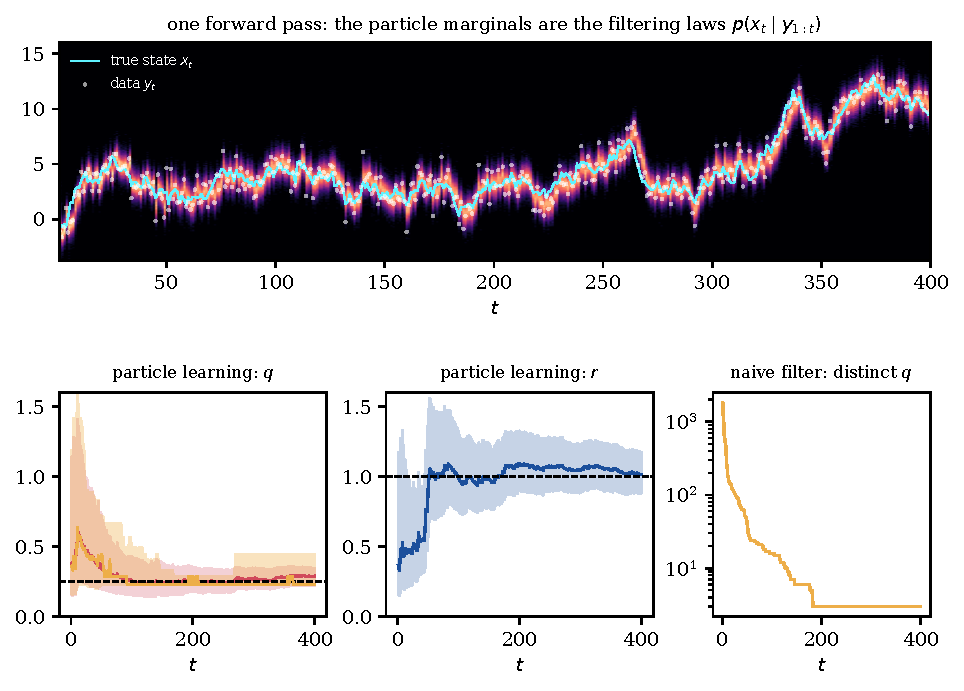
\includegraphics[width=\textwidth]{particle_learning}
\caption{Particle learning with $N = 5000$ particles for the local level model with unknown variances. Top, the particle histograms at each time from one forward pass, which are the filtering laws $p(x_t\mid y_{1:t})$, with the true state and the data. Bottom left and middle, sequential posterior medians and $90\%$ bands for $q$ and $r$, with the true values dashed; the lighter median and band at left are those of the naive filter for $q$. Bottom right, on a logarithmic scale, the number of distinct values of $q$ in the naive filter, which collapses to three.}
\label{fig:pl}
\end{figure}

Carvalho, Johannes, Lopes and Polson~\cite{cjlp2010} extend particle learning to smoothing by backward resampling, in the manner of Godsill, Doucet and West~\cite{gdw2004}, and to sequential model comparison through the predictive likelihoods computed in step one, whose running product is a particle estimate of the marginal likelihood. Carvalho, Lopes, Polson and Taddy~\cite{clpt2010} extend it to general mixtures and nonparametric mixtures. Its precursors are the sufficient statistic filters of Storvik~\cite{storvik2002} and Fearnhead~\cite{fearnhead2002}. In the language of this book, particle learning applies to filtering the lesson of the moment conditioning chapter, Chapter~\ref{ch:types}: carry the conditional sufficient statistics, the macroscopic variables, and let the remaining randomness be regenerated from its exact conditional law. In the language of de Finetti, when the observations are conditionally independent given $\theta$ the conditional sufficient statistic is the summary of the past through which the mixing variable $\theta$ is learned, and the particle carries the same summary in the presence of hidden states.


\section{Kurtz and Xiong: particle representations of filtering equations}
\label{sec:kurtz_xiong}

The particle filter is an algorithm, but it also suggests a theorem: the filtering distribution itself should be the limit of an interacting particle system, and the nonlinear filtering equations should be equations for the de Finetti measure of that system. Kurtz and Xiong made this precise~\cite{kurtzxiong1999}. They consider an infinite system of exchangeable particles $X_i(t)$ with weights $A_i(t)$, driven by individual Brownian motions $B_i$ and by a common noise $W$ shared by all particles, and interacting through their weighted empirical measure. A system of this kind has the form
\[
\begin{gathered}\dd X_i = \sigma(X_i,V)\dd B_i+b(X_i,V)\dd t+\alpha(X_i,V)\dd W,\\ \dd A_i = A_i\big(\beta(X_i,V)\dd t+\gamma(X_i,V)\cdot\dd W\big),\end{gathered}
\]
where the coefficients depend on the weighted empirical measure
\[
V(t) = \lim_{n\to\infty}\frac1n\sum_{i=1}^nA_i(t)\,\delta_{X_i(t)}.
\]
The limit exists because the particles are exchangeable, by de Finetti's theorem and the law of large numbers, and it is a random measure because the particles share the common noise $W$. Kurtz and Xiong show that $V$ is the unique solution of a nonlinear stochastic partial differential equation, and give conditions under which $V$ has an $L^2$ density with respect to Lebesgue measure. In the filtering application the common noise is the observation process and the weighted empirical measure is the filter. It is the unnormalized filter, which solves the linear Zakai equation, when the weights are the Kallianpur Striebel likelihood ratios, and the normalized filter, which solves the nonlinear Kushner Stratonovich equation, when the coefficients of the weights depend on $V$. For the filtering equation, uniqueness follows from uniqueness for the infinite particle system together with uniqueness for a corresponding linear stochastic partial differential equation~\cite[Chapter~7]{xiong2008}. With no common noise and constant weights the system reduces to the McKean Vlasov particle system of Chapter~\ref{ch:kinetic}, and $V$ is its deterministic limit.

The Kurtz Xiong representation closes a circle in this book. In Chapter~\ref{ch:axioms} propagation of chaos was a de Finetti statement: the empirical measure of an exchangeable system converges to a deterministic limit. In Chapter~\ref{ch:kinetic} that limit solved the Boltzmann or McKean Vlasov equation. Here the empirical measure converges to a random limit, because the particles share a common noise, and the limit solves a stochastic equation, the equation of the filter. The particle filter is a finite truncation of the Kurtz Xiong system with resampling in place of continuous weights, and its Monte Carlo error is the error of replacing a de Finetti limit by a finite empirical measure. Xiong's monograph~\cite{xiong2008} develops the filtering theory from this point of view, using the particle representation of the filter to prove uniqueness for the filtering equation and to construct numerical schemes~\cite[Chapters~7 and~8]{xiong2008}. Kurtz and Xiong~\cite{kurtzxiong2001} derived error bounds for such a simulation scheme that account for both the finite number of particles and the Euler discretization of the particle motions.

\subsection{Markov switching filtering equations}

The Kurtz Xiong representation extends to signals that switch between regimes. Give each particle, besides its position and weight, its own copy of a latent regime $z$ that mixes across processes, and let the coefficients of its motion and of its weight depend on that regime. When $z$ is static the result is a mixture of Kurtz Xiong systems. When $z$ is a Markov chain the result is a Markov switching system. Johannes, Polson and Stroud~\cite{jps2009} use particle filters for jump diffusion models of asset prices observed at discrete times, in which each particle carries the latent state variables.

Let $z_t$ be a Markov chain on $\{1,\dots,K\}$ with generator $Q = (Q_{jk})$, and let the signal and observation be
\[
\dd X_t = b(X_t,z_t)\dd t+\sigma(X_t,z_t)\dd B_t,\qquad\dd Y_t = h(X_t,z_t)\dd t+\dd W_t,
\]
where $B$ and $W$ are independent Brownian motions that are independent of $z$. For each regime $k$ let $\mathcal{L}_k f = b(\cdot,k)\cdot\nabla f+\frac12\tr(\sigma\sigma^\top(\cdot,k)\nabla^2f)$ be the generator of the signal frozen in regime $k$. The pair $(X_t,z_t)$ is a Markov process with generator
\[
\mathcal{L}f(x,k) = \mathcal{L}_kf(\cdot,k)(x)+\sum_jQ_{kj}\big(f(x,j)-f(x,k)\big).
\]

\begin{proposition}[Markov switching Zakai equation]
\label{prop:msw_zakai}
Let $b$ and $\sigma$ be Lipschitz and $h$ bounded, and let $\rho_t$ be the unnormalized conditional law of $(X_t,z_t)$ given $\mathcal{F}^Y_t$, defined by the Kallianpur Striebel formula, so that the Zakai equation $\dd\rho_t(f) = \rho_t(\mathcal{L}f)\dd t+\rho_t(hf)\dd Y_t$ holds for $f$ in the domain of $\mathcal{L}$. Write $\rho^k_t(\varphi) = \rho_t(\varphi\otimes\delta_k)$. Then for every $\varphi\in C^2_b(\R^d)$ and $k = 1,\dots,K$,
\[
\dd\rho^k_t(\varphi) = \Big(\rho^k_t(\mathcal{L}_k\varphi)+\sum_jQ_{jk}\,\rho^j_t(\varphi)\Big)\dd t+\rho^k_t\big(h(\cdot,k)\varphi\big)\dd Y_t.
\]
If $\rho^k_t$ has a density $q_t(\cdot,k)$ that is regular enough to integrate by parts, then $(q_t(\cdot,1),\dots,q_t(\cdot,K))$ solves the coupled system
\[
\begin{aligned}\dd q_t(\cdot,k) &= \Big(\mathcal{L}_k^*q_t(\cdot,k)+\sum_{j}Q_{jk}\,q_t(\cdot,j)\Big)\dd t\\ &\quad+h(\cdot,k)\,q_t(\cdot,k)\,\dd Y_t,\qquad k = 1,\dots,K,\end{aligned}
\]
where $\mathcal{L}_k^*$ is the formal adjoint of $\mathcal{L}_k$. The filtering distribution of the state is the mixture $\pi_t(\dd x) = \sum_kq_t(x,k)\dd x\big/\sum_k\int q_t(x',k)\dd x'$, and the regime probabilities are $\P(z_t = k\mid\mathcal{F}^Y_t) = \int q_t(x,k)\dd x\big/\sum_j\int q_t(x,j)\dd x$.
\end{proposition}

\begin{proof}
Apply the Zakai equation to $f(x,j) = \varphi(x)\delta_{jk}$. Because $\sum_lQ_{jl} = 0$, $\mathcal{L}f(x,j) = \delta_{jk}\mathcal{L}_k\varphi(x)+Q_{jk}\varphi(x)$. Hence $\rho_t(\mathcal{L}f) = \rho^k_t(\mathcal{L}_k\varphi)+\sum_jQ_{jk}\rho^j_t(\varphi)$ and $\rho_t(hf) = \rho^k_t(h(\cdot,k)\varphi)$, which is the first display. If $\rho^k_t$ has density $q_t(\cdot,k)$, then $\rho^k_t(\mathcal{L}_k\varphi) = \int\varphi\,\mathcal{L}_k^*q_t(\cdot,k)\dd x$ by integration by parts, which gives the coupled system. The last two statements are the Kallianpur Striebel normalization, $\pi_t(\varphi) = \sum_k\rho^k_t(\varphi)/\sum_k\rho^k_t(1)$.
\end{proof}

Each regime component evolves by its own Zakai equation, and the components exchange mass at the rates of the regime chain. This is the Markov switching stochastic partial differential equation. Its particle representation follows the Kurtz Xiong recipe with the regime added to the particle's state: particle $i$ carries $(X_i,Z_i,A_i)$, where $(X_i,Z_i)$ is an independent copy of the signal, with $Z_i$ a copy of the regime chain and $X_i$ moving with the coefficients of regime $Z_i$, and the weight evolves by $\dd A_i = A_i\,h(X_i,Z_i)\dd Y_t$. The weighted empirical measure
\[
V_t = \lim_{n\to\infty}\frac1n\sum_{i=1}^nA_i(t)\,\delta_{(X_i(t),Z_i(t))}
\]
equals $\rho_t$. Under the reference measure in which $Y$ is a Brownian motion independent of the signal, the triples $(X_i,Z_i,A_i)$ are independent given $Y$, and the Kallianpur Striebel formula gives $\E[f(X_i(t),Z_i(t))A_i(t)\mid Y] = \rho_t(f)$, so the limit exists and equals $\rho_t$ by the law of large numbers conditional on $Y$. After normalization by $V_t(1)$, its marginal on the regimes gives the regime filter and its marginal on the states gives the state filter. In discrete time, with resampling in place of continuous weights, it becomes a particle filter for a Markov switching model.

Figure~\ref{fig:msw} shows a two regime example in discrete time, with steps of length $0.05$ at which the particles are propagated, weighted and resampled as in the bootstrap filter. In regime zero the state drifts upward at rate one with volatility $0.6$, and in regime one it drifts downward at rate one with volatility $1.6$. The chain leaves regime zero at rate $0.15$ and regime one at rate $0.25$ per unit time, and the state is observed at every step with noise of standard deviation $0.3$. The lower panel shows the regime probability $\P(z_t = 1\mid y_{1:t})$, read off as the total weight of the particles in regime one. The filter classifies the regime correctly at $93\%$ of the steps. The path has two switches, and the filter registers them after $0.4$ and $0.65$ time units, a delay that accounts for about half of the misclassified steps. The rest are brief excursions of the filtered probability across one half, in both regimes.

\begin{figure}[t]
\centering
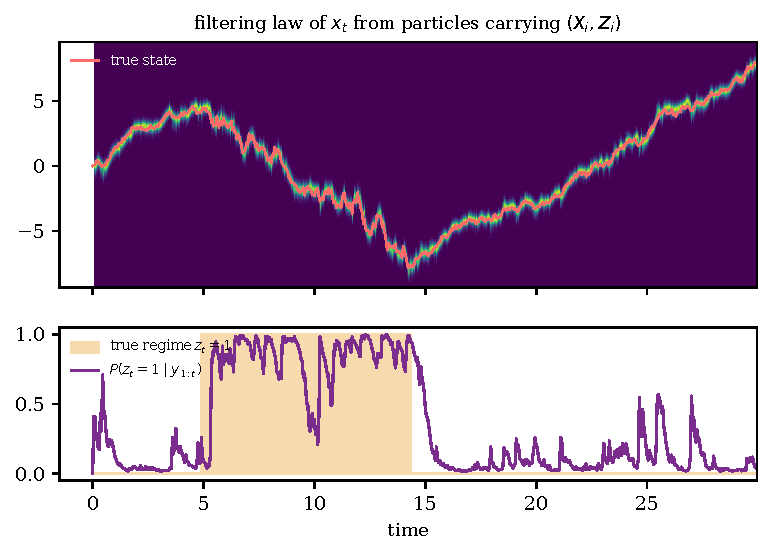
\includegraphics[width=0.95\textwidth]{markov_switching}
\caption{A Markov switching filter with $N = 4000$ particles, each of which carries its own latent regime chain. Top, the filtering law of the state with the true path. Bottom, the filtered regime probability against the true regime (shaded).}
\label{fig:msw}
\end{figure}
